\documentclass{article}


\usepackage[french]{babel}
\usepackage[utf8]{inputenc}

\usepackage[a4paper,top=2cm,bottom=2cm,left=3cm,right=3cm,marginparwidth=1.75cm]{geometry}


\usepackage{amsmath}
\usepackage{graphicx}
\usepackage[colorlinks=true, allcolors=blue]{hyperref}
\usepackage{caption}
\usepackage{listings}

\title{Première version du cahier d’analyse des besoins à propos d'un programme de jeux d'échecs}
\author{Rossignon Morgan, Daniel Karl, Salomode Florian, Beites Marvin, Zucchelli Thomas}

\begin{document}

\maketitle
\centerline{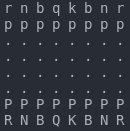
\includegraphics[scale = 1]{img/echecs_title.png}}

\tableofcontents
\newpage

\section{Objectifs généraux du projet}
Le but du projet est de programmer un joueur d'échec complet en appliquant les algorithmes les plus fréquents et en utilisant au mieux les bitboards qui sont un moyen de représenter l'échiquier à l'aide de douze variables de 64bits chacune (comme le nombre de case d'un échiquier). \newline
Ces  douze variables, une pour chaque type de pièces par couleur stockent donc les positions des différentes pièces du plateau de jeu. Le site suivant l'explique d'ailleurs de manière précise \cite{Bitboards}. 

L'interface utilisateur sera purement en mode texte (ce n'est pas le but du projet). Si possible, plusieurs approches pourront être implantées et comparées via des tournois entre les différentes stratégies.

Le projet se dirigera vers des techniques d'exploration d'arbre classiques telles que Minimax-
ab \cite{Minmax-ab}, Negamax \cite{Negamax}, Negascout \cite{Negascout}, MTD(f) \cite{MTD(f)}, Monte-Carlo Tree Search (MCTS)\cite{MCTS}. Ainsi qu'au développement d'heuristiques propres au jeu dans l'idée d'éliminer le plus efficacement les branches "perdantes" \cite{Heuristiques}.


\section{Analyse de l'existant}
Il est possible de trouver le pseudo-code et le principe de fonctionnement des algorithmes Minimax-
ab \cite{Minmax-ab}, Negamax \cite{Negamax}, Negascout \cite{Negascout}, MTD(f) \cite{MTD(f)}, Monte-Carlo Tree Search (MCTS)\cite{MCTS} sur internet, ces pseudo-codes sont disponibles en annexe.
\newline
Afin de discuter du fonctionnement de l'algorithme Minimax-ab il faut parler du fonctionnement de l'algorithme Minimax.
\newline
L'algorithme Minimax a pour but de trouver la liste des meilleurs coups à jouer, pour cela on va générer tous les coups possibles dans un arbre jusqu'à une certaine profondeur,  puis en partant des feuilles en remontant jusqu'à la racine on remonte alternativement le meilleur coup favorisant notre victoire et le meilleur coup favorisant le coup de notre adversaire\cite{Heuristiques}.
\newline\newline
L'algorithme Minimax-ab a le même principe à la différence que lorsqu'il remonte l'arbre des coups possibles il ne prend pas en la peine de juger l'efficacité de certains coups en fonction des autres coups qu'il a déjà jugé plus efficace, au travers d'une comparaison entre deux variables, alpha et bêta\cite{Heuristiques}.
\newline\newline
L'algorithme Negamax se différencie de l'algorithme Minimax-ab par le fait que plutôt que de maximiser le coup du joueur et minimiser le coup de l'adversaire il inverse le signe des évaluations à chaque niveau de profondeur de l'arbre de décision et ne cherche plus qu'à maximiser la valeur du coup à évaluer\cite{Negamax}.
\newline\newline
Avec l'algorithme Monte-Carlo Tree Search, un nœud de l'arbre de décision correspond à un état du jeu mais possède aussi deux valeurs, le nombre de simulations gagnantes et le nombre de simulations totales sur la branche.
L'algorithme fonctionne en quatre étapes\cite{MonteCarlo}:
\begin{itemize}
\item La sélection successive des enfants de la racine jusqu'à atteindre une feuille.
\item L'expansion de l'arbre, en ajoutant un enfant à la feuille si celle-ci n'est pas finale.
\item La simulation d'une partie au hasard depuis l'enfant rajouté jusqu'à atteindre une fin de partie.
\item La remontée du résultat de la partie par la mise à jour du nombre de simulation victorieuse et du nombre de simulation totale pour chaque nœuds.
\end{itemize}
\newpage
\centerline{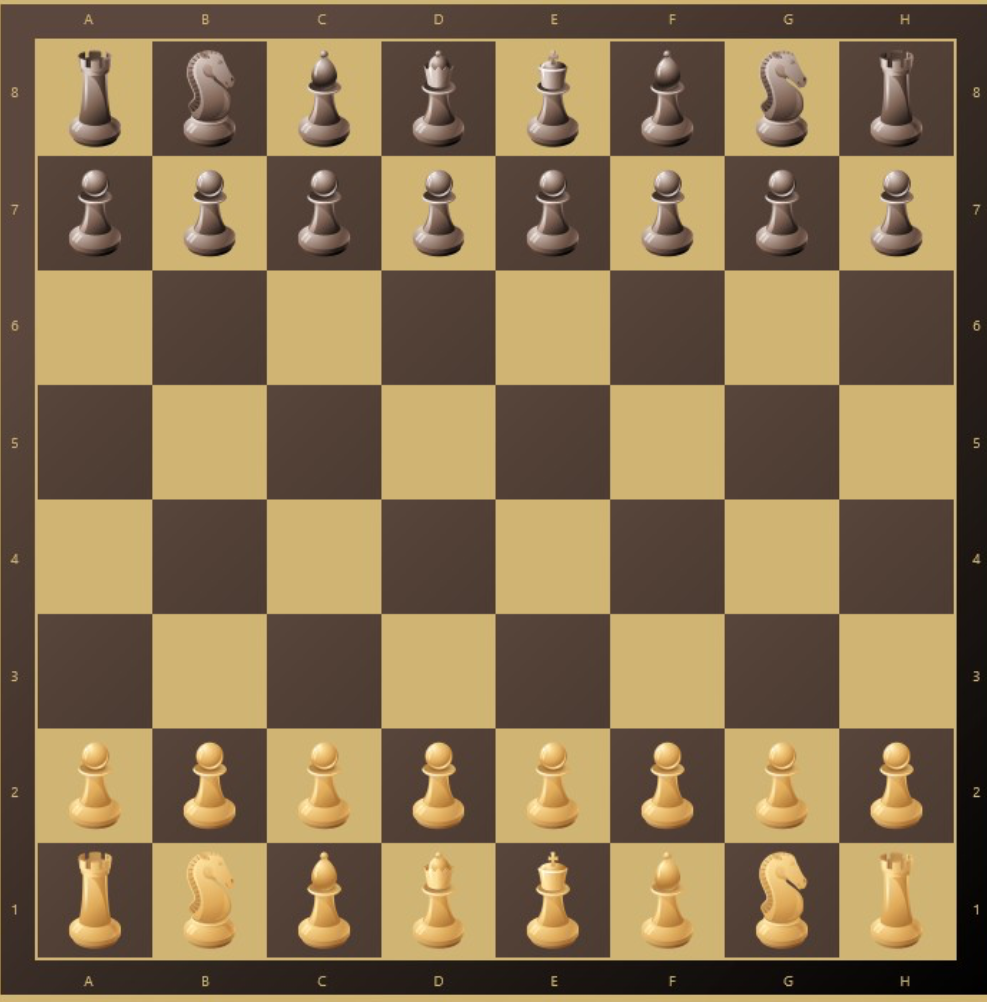
\includegraphics[scale = 0.25]{img/Echiquier.png}}
La plupart des logiciels de jeu d'échecs proposés au grand public, disponibles dans les boutiques virtuelles comme le Microsoft store, optent pour un affichage graphique afin de jouer aux échecs, toutefois on peut se rendre compte que ces logiciels permettent aux joueurs de :
\begin{itemize}
\item sélectionner qui joue en premier. (qui joue les pièces blanches)
\item sélectionner le nombre de joueurs. (l'ia contre l'ia, 1 joueur contre l'ia ou 2 joueurs)
\item sélectionner une difficulté pour l'ia.
\newline{
\includegraphics[scale = 0.5]{img/Computer_level.png}}
\item visualiser les mouvements d'une pièce
\newline
\centerline{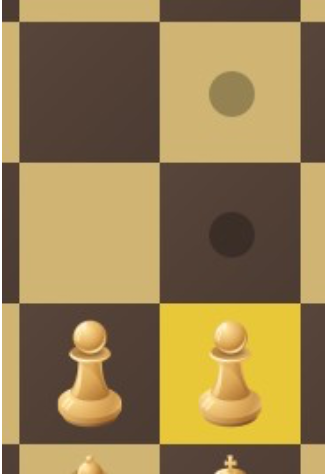
\includegraphics[scale = 0.5]{img/Piece_move.png}}
\item sauvegarder une partie pour la reprendre plus tard. -charger une partie sauvegardée.
\newline\newline
\end{itemize}
Mais il existe également des logiciels, quant-à eux plus scientifique, avec pour vocation d'exercer  des algorithmes contre des champions humains ou contre d'autres logiciels.
\newline
C'est le cas de Kaissa qui fût le premier programme à avoir gagné le championnat ACM d'échecs informatiques de 1974. Ce dernier utilise un algorithme Minimax alpha beta \cite{KaissaAB} pour calculer ses coups et un système de bitboard pour déterminer les mouvements légaux d'une pièce \cite{KaissaBitboard}.
\newline
Nous pouvons cité Deep Thought qui remporta le 19ème championnat ACM d'échecs informatiques, il s'agit du premier ordinateur avec le niveau d'un grand maître et joua contre Garry Kasparov en 1989 et fut battu\cite{Deep}. 
\newline
Jusqu'à Deep Blue qui possède une puce lui permettant de paralléliser l'algorithme de recherche alpha-bêta\cite{DeepSystem} et fut le premier ordinateur à avoir battu Kasparov en 1996\cite{Deep}.
\newpage
\section{Description des besoins}

%Éventuellement avec distinction besoins
%utilisateurs/besoins système.

%Ces besoins seront expliqués, justifiés, illustrés au moyen de : scénarios,
%prototypes (par ex. prototypes papier pour les interfaces, prototypes
%implémentés pour la faisabilité)
\begin{itemize}

\subsection{Liste des besoins fonctionnels}
\medskip
%chacun associés à :
%- Un niveau de priorité d’implémentation dans le projet.
%- Toutes ou une partie des rubriques (a)-(e) ci-dessous.

%Analyse de source (lecture de fichier ?...), récupération des graphes de dépendances (ou création suite à l'analyse de source ?...),  affichage des graphes.
    \item \textbf{Création du plateau de jeu : }
    \medskip
    \begin{itemize}
        \item Représentation du plateau à l'aide de bitboards \cite{Bitboards}, chaque bitboard représentera l'emplacement des pièces d'un même type et d'une même couleur. ( c-a-d qu'il y aura un bitboard pour l'emplacement de tous les pions blanc, un bitboard pour l'emplacement de tous les Cavaliers blanc,...).
    \end{itemize}
    \medskip
    \item \textbf{Afficher le plateau de jeu : }
    \medskip
    \begin{itemize}
        \item Affichage en texte, une lettre représente un pion (p = pion, k = roi, q = reine,
        b = fou, r = tour, n = cavalier).
        Les cases vides, quand à elle contiendront un point "." dans un souci de lisibilité.
        \item Afin de différencier les pions des 2 joueurs du plateau de jeu, le joueur blanc aura des pions en majuscule et le joueur noir en minuscule.
        \item Les coordonnées des cases seront les mêmes que sur le jeu d'échec original, les numéros représentent les lignes et les lettres pour les colonnes, par exemple (a1 = 1ère case en bas à gauche \dots).
    \end{itemize}
    \centerline{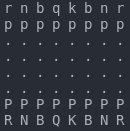
\includegraphics[scale = 0.5]{img/echecs_title.png}}
    \medskip
    \item \textbf{Lister les mouvements possibles : }
    \newline
    En cas de jeu de l'utilisateur contre un des différents algorithmes, une commande "playable" permet d'afficher la liste de tous les coups jouables pour l'utilisateur ( par exemple : h2h4 \dots).
    \newline
    \centerline{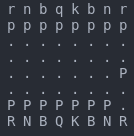
\includegraphics[scale = 0.5]{img/chess_moveh2h4.png}}
    \medskip
    \item \textbf{Déplacer une pièce : }
    \newline
    Le programme doit faire respecter les règles du jeu aux différents algorithmes, ou joueur humain.
    Le déplacement d'une pièce doit vérifier au préalable que le mouvement est possible, et si c'est le cas, ce que ce mouvement engendre.
    \begin{enumerate}
        \item Le programme doit vérifier que le mouvement demandé correspond à un des mouvements possibles de la pièce.
        Suivant les pièces : 
        \begin{itemize}
            \item \textbf{Pion (p,P) : } Le pion avance d'une case en ligne droite uniquement (ni sur les cotés ni en arrière) hormis le premier déplacement de chaque pions qui peut être de 1 ou 2 cases au choix.
            Le pion peut aussi "manger" une pièce, dans ce cas le déplacement se fait en diagonale d'une portée de 1, avec la aussi une situation particulière, le "En passant"
            \item \textbf{Roi (k,K) : } Le roi peut aller dans toutes les directions mais d'une seule case.
            \item \textbf{Reine (q,Q) : } La reine peut aller dans toutes les directions et n'est pas limitée par le nombre de cases de déplacement.
            \item \textbf{Fou (b,B) : } Le fou se déplace uniquement en diagonale et n'est pas limité par le nombre de cases de déplacement.
            \item \textbf{Tour (r,R) : } La tour est le complémentaire du fou, elle se déplace uniquement en ligne horizontale ou verticale sans limitation du nombre de cases de déplacement.
            \item \textbf{Cavalier (n,N) : } Le cavalier à le déplacement le plus atypique, il peux sauter au dessus des autres pièces durant son déplacement, il se déplace en "L" dans le sens qu'il veut.
            \newline
            \centerline{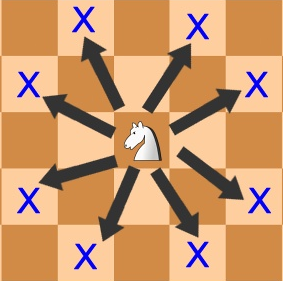
\includegraphics[scale = 0.2]{img/Deplacement_cavalier.png}}
        \end{itemize}
        \item Si le mouvement est correct pour la pièce, il doit vérifier que la case ou le chemin venant vers la case n'est pas occupé par une pièce alliée (hormis le cavalier qui doit juste vérifier la case d'arrivée), auquel cas, le mouvement n'est pas valide.
        \item Si la case n'est pas occupée par une pièce alliée, le programme vérifie si une pièce ennemie se trouve sur la case.
        Si c'est le cas la pièce ennemie est détruite du plateau de jeu.
        A noter que le pion ne "mange" pas de la même façon qu'il se déplace, en effet il ne peut manger qu'en diagonale à distance de 1.
        \item Enfin, la pièce se déplace sur la case cible.
        À noter que si un pion se retrouve au bout de l'échiquier la pièce doit pouvoir être changer en la pièce du choix de l'IA / l'utilisateur.
    \end{enumerate}
    \medskip
    \item \textbf{Garder une trace de l'historique : }
    \newline
        Le programme doit garder en mémoire les 6 derniers plateaux de jeux (3 derniers coups de chaque joueurs) afin de les comparer et d'annoncer un match nul si le même plateau est répété 3 fois. 
    \medskip
    \item \textbf{Choisir les algorithmes à utiliser : }
        \newline
        En début de partie, une liste des différents algorithmes est proposée à l'utilisateur qui n'a plus qu'à recopier dans le terminal celle contre qui il veut jouer ou tout simplement celles qu'il veut voir s'affronter, ainsi que ses paramètres ( profondeur de recherche, attribution des rôles Joueur\_1 et Joueur\_2 \dots).
    \medskip
    \item \textbf{Afficher des statistiques :
    }
        \newline
        Le logiciel doit pouvoir afficher les statistiques de la dernière partie lancée. 
        \newline
        Il faudra donc que le logiciel affiche le type d'algorithme utilisé et ses paramètres, quelle ia a gagné ou non, le nombre de tours pour finir la partie, pour chaque tour le temps pris par les ia ou joueurs pour réaliser une action, et le temps moyen d'un tour des ia.
    \medskip
    \item \textbf{Lancer un tournoi entre algorithmes : }
    \newline
        Il est possible de lancer un tournoi entre différents algorithmes afin de voir lequel est le plus performant en rajoutant l'option "-tournament NAME" à l'appel du logiciel.
        Le tournoi serait une forme de "ligue" ou chaque algorithme jouerait 2 fois contre tous les autres, une fois en tant que joueur blanc une fois en tant que joueur noir.
        \newline
        À la suite de ce tournoi, les informations suivantes sont stockés dans un fichier du même nom que celui du tournoi (NAME) :
        \begin{itemize}
            \item Un classement de tous les algorithmes suivant le nombre de victoires et basé surtout sur le nombre de coups joués jusqu'à la victoire.
            \item Un cour résumé sur chaque match de la forme suivante " Minmax-ab Blanc 1 MCTS Noir 0 36cp" qui signifie ici une victoire de minmax-ab sur MCTS en 36 coups.
            \newline
            \centerline{
\includegraphics[scale = 0.5]{img/Summarytournament.png}}
        \end{itemize}
    \medskip
    \item \textbf{Lancer des Algorithmes sur des énigmes : }
    \newline
        Dans le monde des Échecs il existe des "problèmes" d'échec \cite{Krt}, c-à-d d'après un plateau donné il faut réussir à mettre en place des stratégies comme mettre le roi adverse en échec et mat en un certain nombre de coups.\newline
        \begin{itemize}
            \item Les énigmes sont stockées dans le dossier enigm dans un fichier au nom de l'énigme comme l'exemple suivant : \newline
            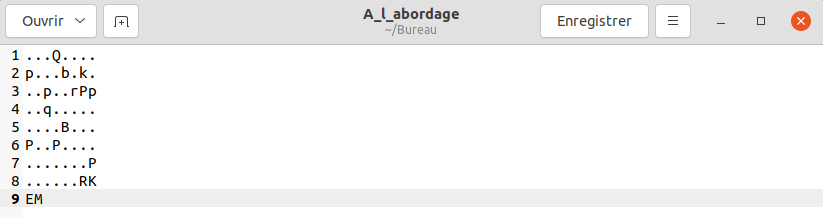
\includegraphics[scale = 0.3]{img/a_l_abordage.png}
            \item Dans les fichiers enigm/*, à la suite de l'échiquier de départ se trouve les conditions de victoires de l'énigme : "EM" pour un echec et mat, "EMC5" Si il faut un echec et mat en moins de 5 coups \dots
        \end{itemize}
        Les options -Enigm list affichent la liste des noms des énigmes connu par le programme.
        il sera donc possible de lancer les algorithmes sur ces "problèmes".
        Les problèmes nécessitent un joueur adverse, le programme utiliseras donc l'algorithme de MCTS en second joueur.
        Le programme doit donc générer la partie selon le modèle de l'énigme.
\end{itemize}



\subsection{Liste des besoins non-fonctionnels}
\medskip
\begin{itemize}
    
    \item \textbf{Performances : }
    Une partie jouée entre deux Algorithmes ne doit pas non plus durer des heures, les algorithmes ne devrons pas dépasser un certain temps pour chaque coup.
    \newline
    \item \textbf{Facilité d'utilisation : } 
    Toutes les commandes possibles doivent être listées à l'utilisateur, ainsi que leurs fonctions, afin de le guider et qu'il ne perde pas de temps à comprendre le fonctionnement du programme.
    \newline
    \item \textbf{Domaine d'action : } 
    Les utilisateurs seront des informaticiens. Le programme étant basé avant tout sur l'interaction d'une IA contre une autre plutôt que du joueur contre une IA.
    \newline
    \item \textbf{Portabilité : } 
    \newline
    Le programme doit être exécutable sous les systèmes d'exploitation suivantes : Ubuntu 20.04, Ubuntu 21.10 ainsi que sur mac OS Catalina.
    \newline
    
\end{itemize}
\medskip
\section{Idée de structure}
Pour l'instant, nous avons une réflexion sur 2 partie de structure. (En cours de travail) \newline
\begin{itemize}
    \item Une partie Jeu de base :\newline
    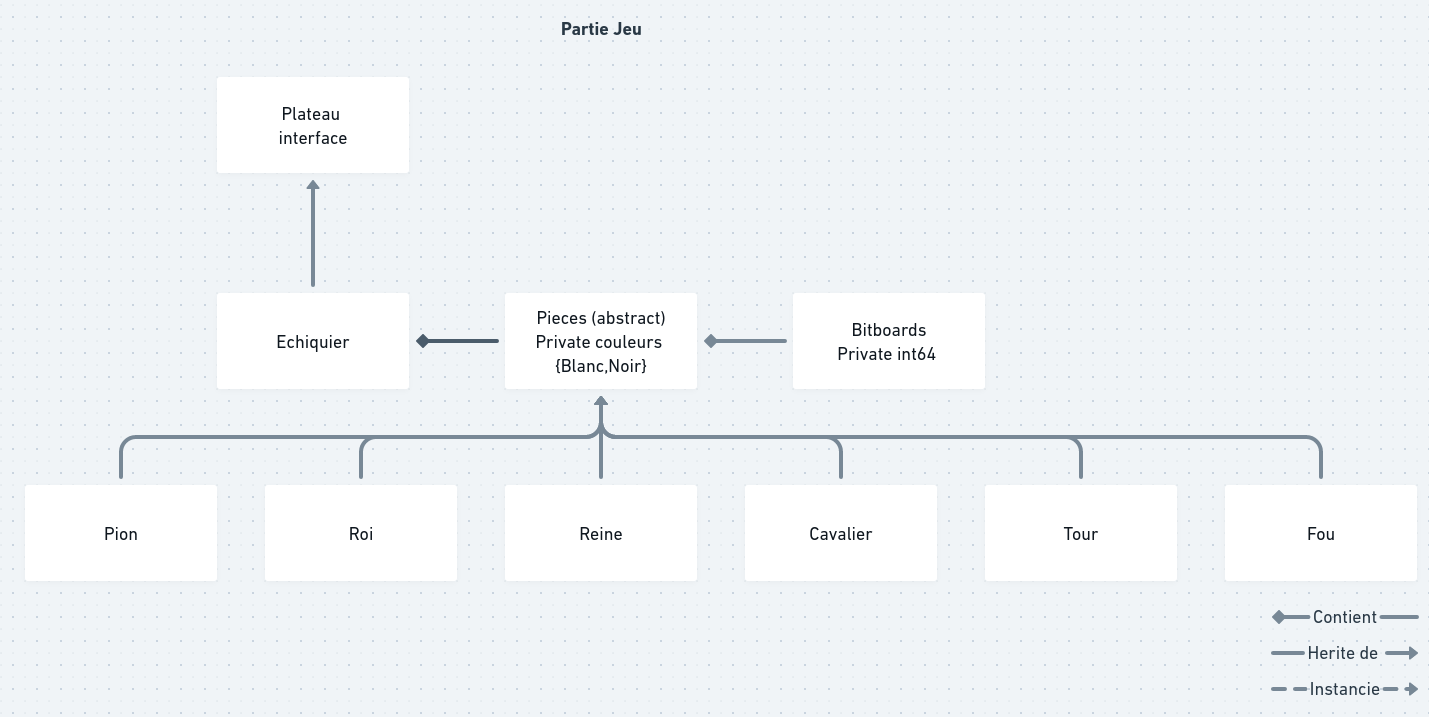
\includegraphics[scale = 0.3]{img/UML_part_gaming_chess.png}
    \newpage
    \item Une partie avec l'abstract factory permettant de générer les différentes "IA" : \newline
    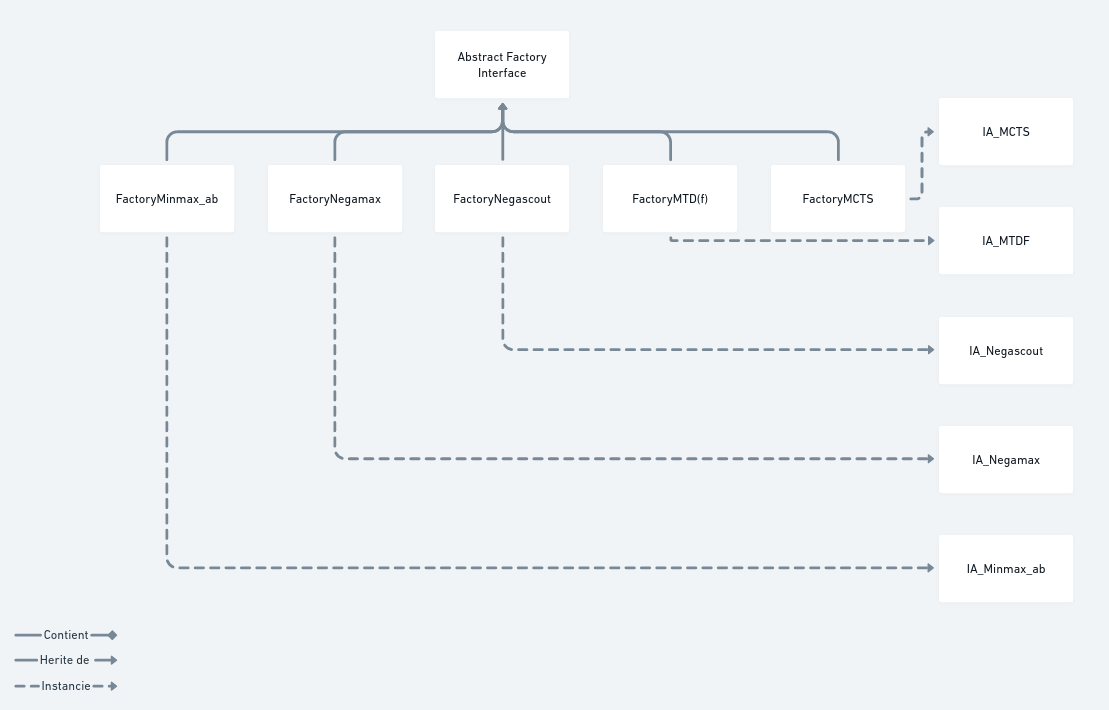
\includegraphics[scale = 0.4]{img/Abstract_factory_IA_chess.png}
    
\end{itemize}
\section{Liste des outils}
\begin{itemize}
    \item Langage à utiliser : C++
    \item Utilisation de Bitboards pour représenter et gérer les pièces.
\end{itemize}
\section{Annexe}
\subsection{Pseudo-code des différentes techniques d'exploration d'arbre classiques : }
\medskip
\subsubsection{Minmax-ab :}
\centerline{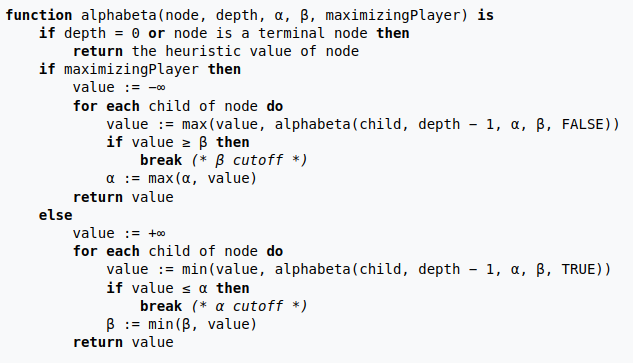
\includegraphics[scale = 0.5]{img/Alpha_beta_minmax.png}}
\medskip
Source pseudo-code Minmax-ab \cite{Minmax-ab_pc}.
\subsubsection{Negamax : }
\centerline{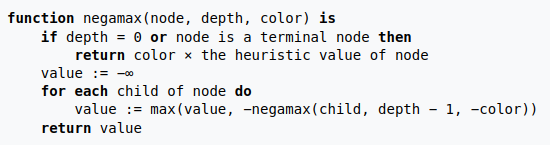
\includegraphics[scale = 0.5]{img/Negamax_1.png}}
\centerline{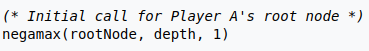
\includegraphics[scale = 0.5]{img/Negamax_2.png}}
\centerline{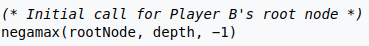
\includegraphics[scale = 0.5]{img/Negamax_3.png}}
\medskip
Source pseudo-code Negamax \cite{Negamax_pc}.
\subsubsection{Negascout : }

\centerline{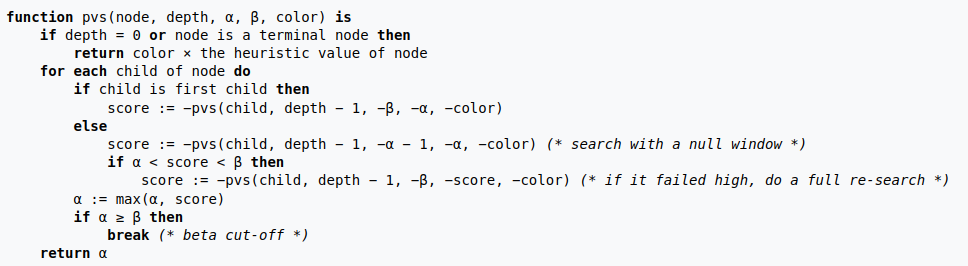
\includegraphics[scale = 0.5]{img/Negascout.png}}
\medskip
Source pseudo-code Negascout \cite{Negascout_pc}.
\subsubsection{MTD(f) : }

\centerline{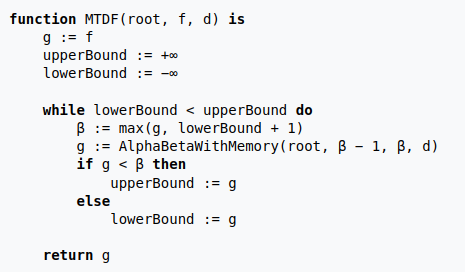
\includegraphics[scale = 0.5]{img/MTDf.png}}
\medskip
Source pseudo-code MTD(f) \cite{MTDf_pc}.
\subsubsection{Monte-Carlo Tree Search (MCTS) : }

\centerline{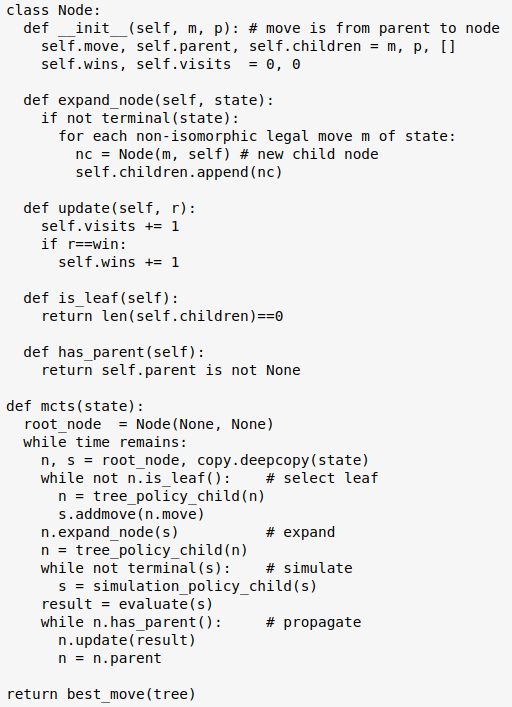
\includegraphics[scale = 0.5]{img/Monte_carlo_tree_search.png}}
\medskip
Source pseudo-code MCTS \cite{MCTS_pc}.
\newpage


\bibliographystyle{unsrt}
\bibliography{sample}

\end{document}